\chapter{Arhitectura platformei}
 Provocarea de a elabora o platformă web destinată atât auditorilor publici cât și reprezentanților instituțiilor din administrația publică  a impus nevoiea de crea o arhitectură dinamică, modulară și usor de mărit în cazul adaugării a noi funcționalități.
 
De asemenea, un număr mare de functionalități necesită implementarea și a diferite \textit{design pattern-uri}, care se asigură că modulule definite comunică într-un mod cât mai eficient între ele și promovează reutilizarea codului deja scris.

Acest capitol incearcă să descrie motivația pentru alegerile făcute în materie de tehnologii folosite pentru a dezvolta componentele cheie ale aplicației: frontend, backend stocarea datelor și câteva aspecte legate de securitatea de bază a platformei.

\section {Arhitectura generală}
Arhitectura generală a fost gândita de la început într-un mod care permite adăugarea de noi funcționalități în aplicație fără a deteriora Structură sau funcționalitățile deja implementate.

Acestea fiind zise, proiectul este împărțit în două mari componente (client și server)  care comunică între ele prin intermediul \textit{request-urilor HTTPS}, și anume:

\begin{itemize}
	
	\item componenta de server, este alcatuită din diferite \textit{endpoint-uri}  Web API care oferă funcționalități clienților săi, aceasta comunicând și cu mediul de stocare al datelor, o bază de date MySQL;
	
	\item componenta client, sau interfața grafică a platformei, este o aplicație web interactivă de tipul SPA (\textit{Single page application}), oferind funcționalitățile descrise prin intermediul \textit{request-urilor} către server, urmând ca mai apoi să fie afișate pe pagina web prin intermediul \textit{WebAssembly-ului}.
\end{itemize}  

\subsection*{Diagrame de context C4 }

Diagramele de context C4 reprezintă un stadard în ceea ce privește o vedere de ansamblu, dar care merge inspectată în detaliu pentru fiecare component al aplicației, astfel promovând o ierarhizarea și o înțelegere a întreg sistemului mai bună.\\


\subsection*{Nivelul 1}
Primnul nivel al diagramelor de context oferă o viziune de ansamblu asupra sistemelor ce compun solutia descrisă.
\vspace{1cm}
\begin{figure}[h]
	\centering
	
	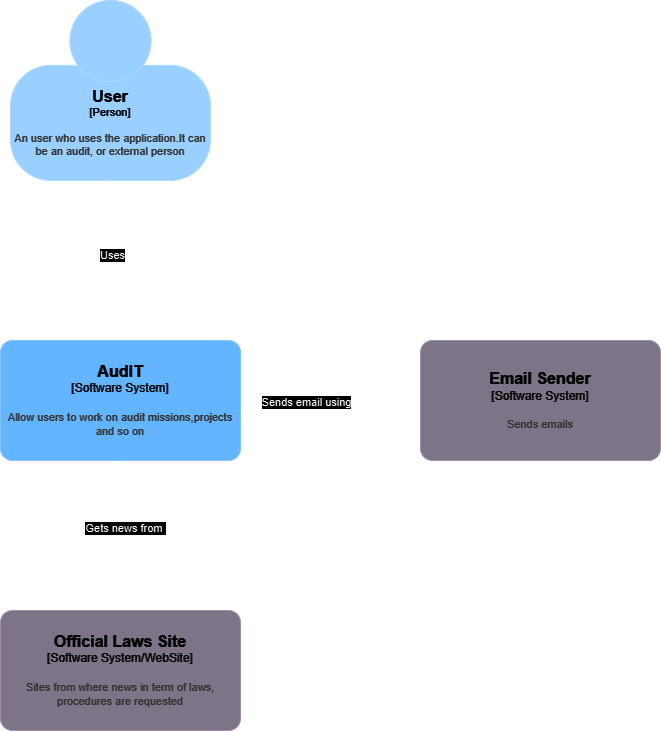
\includegraphics[width=0.6\textwidth]{c2/C4_level1}
	\caption{Primul nivel diagramă C4}
\end{figure}

\newpage
\subsection*{Nivelul 2}
Al doilea nivel prezintă  \textit{containerele} principale ale fiecăurui sistem din nivelul anterior, astfel oferind o viziune mai clară asupra arhitecturii generale a platformei și a funcționalităților sale.
\vspace{1cm}
\begin{figure}[h]
	\centering
	
	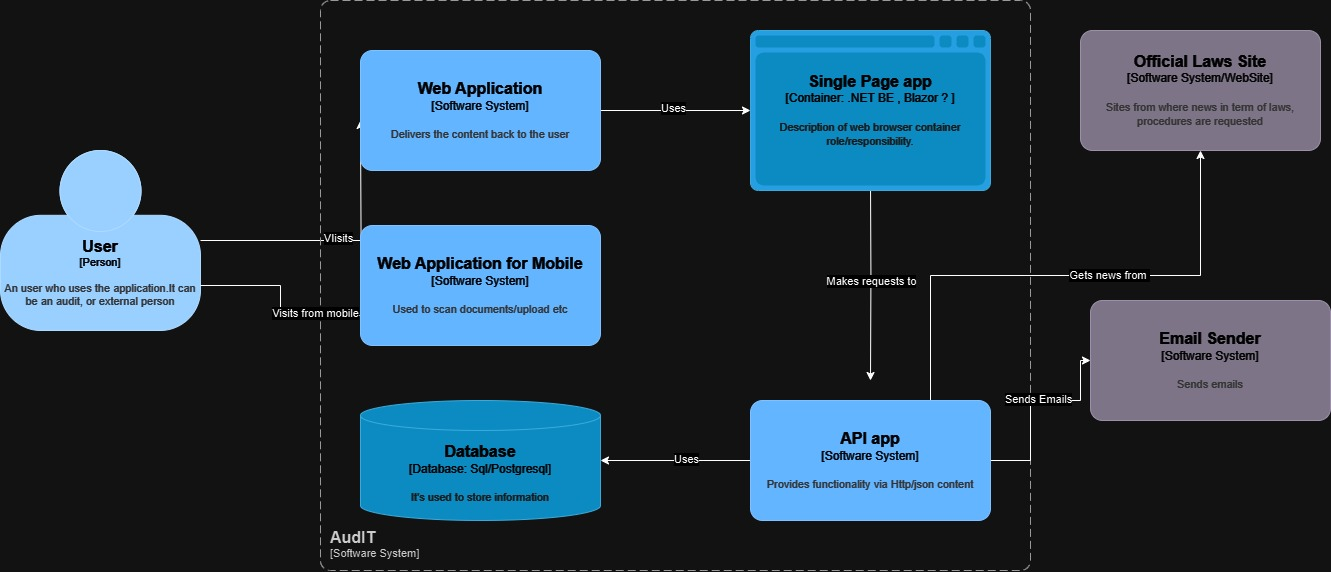
\includegraphics[width=0.7\textwidth]{c2/C4_level2}
	\caption{Al doile nivel din diagrama C4}
\end{figure}

\subsection*{Nivelul 3}
Al treilea nivel oferă o viziune mult mai detaliată asupra componentelor ce aparțin \textit{container-ului} de la nivelul secund, oferind abstractii cât mai apropiate de codul ce urmează a fi scris pentru a le implementa.

\vspace{1cm}
\begin{figure}[h]
	\centering
	
	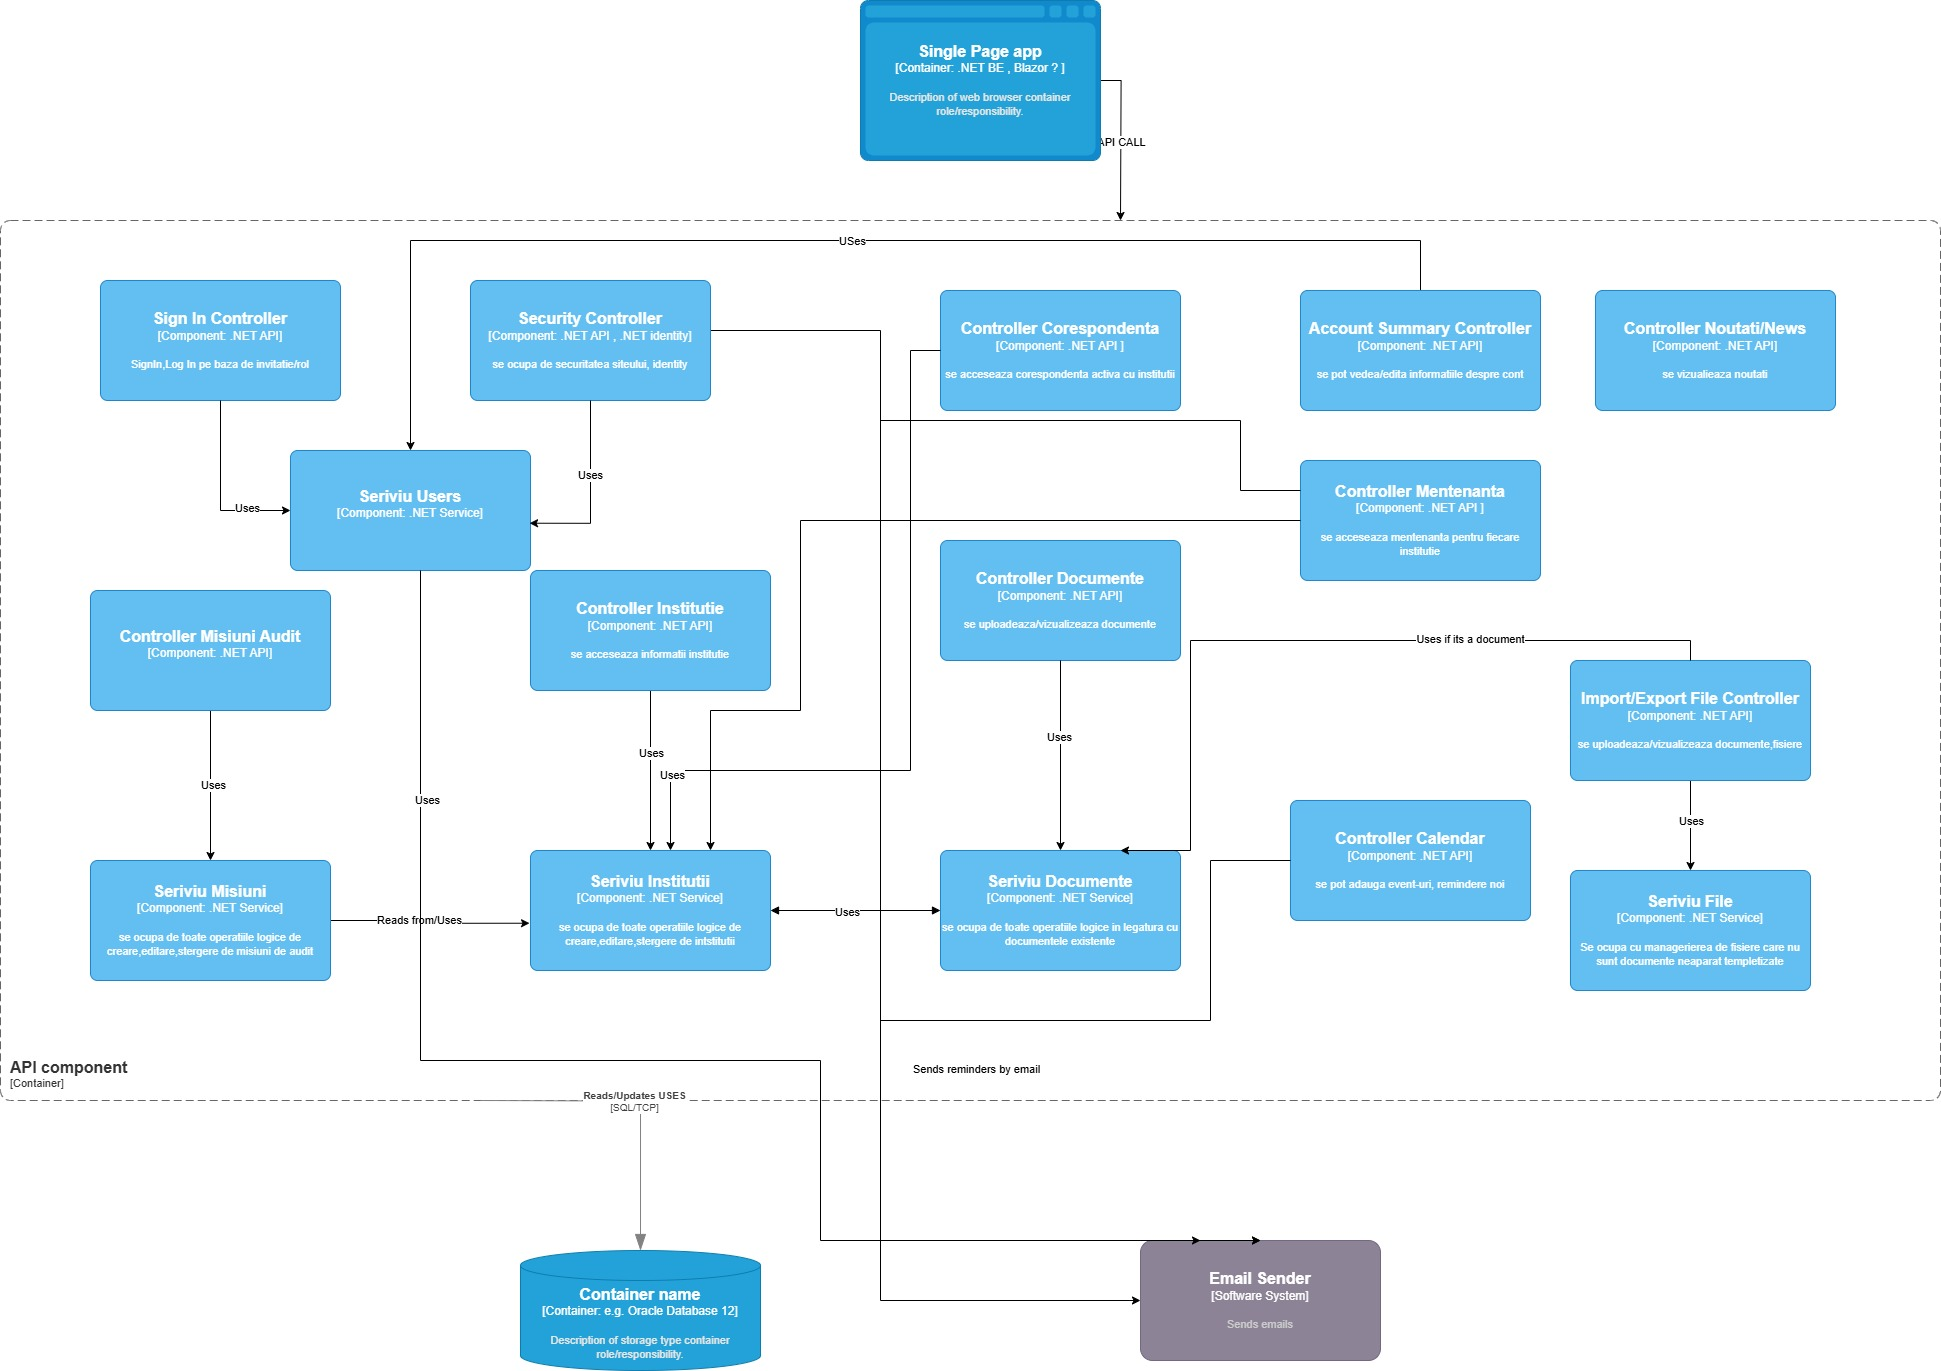
\includegraphics[width=1\textwidth]{c2/C4_level3}
	\caption{Nivelul trei din diagrama C4}
\end{figure}



\section{Arhitectura serverului}

\subsection*{Arhitectura \textit{monolith}}

Arhitectura generală a serverului este una de tip \textit{monolith} tradițional, împartită pe module, cu dependențe slabe între ele, care comunică prin intermediul unor contracte (interfațe) bine definte.

Alegerea acestui tip de arhitectură a fost motivată de mai multe avantaje cheie ale acesteia: 
\begin{itemize}
	\item simplitatea dezvoltării în cadrul arhitecturii de tip monolith permite lucrul pe o singură bază de cod , ceea ce simplică major procesul de dezvoltare, testare și de depistare a erorilor, fiind esențială în fazele de început al unui proiect;
	
	\item  performanța sporită în cadrul unei aplicații care răspunde \textit{request-urilor}, astfel un singur \textit{API} poate răspunde la toate cererile, eliminând nevoia de a activa și alte \textit{API-uri} externe pentru îndeplinirea sarcinii, ca în cazul arhitecturii de micro-servicii;
	
	\item ușurința testării de tip \textit{unit-testing} cât și \textit{integration-testing} întrucat toate modulele sunt în același loc;
	
	\item  depistarea erorilor și rezolvarea lor este mult mai rapidă.
\end{itemize}

Conform oricărei alegeri făcute, trebuie puse în balanță avantajele și dezavantajele pe care această le oferă și  să se compare strict cu nevoile și problemele care se incearcă a se rezolva. Privind în ansamblu și pe termen lung, arhitectura de tip \textit{monolith} prezintă și unele dezavantaje: 

\begin{itemize}

 \item dezvoltarea încetinita în momentul în care funcționalitățile pe care dorim să le implementăm cresc ca și număr, întrucat toate modulele sunt comasate într-un singur loc;
 
 \item \textit{scalabilitate redusă} datorită strânsei legături dintre componentele prezente în aplicație;
 
 \item 	orice schimbare adusă în materie de noi funcționalități necesită lansarea întregii aplicații, nu doar a unui singur modul.

\end{itemize}

Pentru a diminua efectele negative pe care aceste dezavantaje le au asupra întregului proces de dezvoltare a aplicației, s-a încercat implementarea diferitelor soluții în materie de arhitectură,  \textit{desing pattern-uri} creaționale, arhitecturale cât și a numeroase practici bune comune în scrierea și mentenanța codului.

\subsection*{Arhitectura \textit{Clean Code}}
Arhitectura \textit{Clean Code } este bazată pe ideea principală precum că stratul de logică internă (\textit{business layer}) este situat central în diagrama circulară, astfel acesta este protejat de schimbări externe. Această proprietate poate fi reformulată astfel încât se definește \textbf{Regula Dependenței} care presupune că dependențele pot să fie orientate doar înspre interiorul cercului, astfel niciunul din modulele interioare nu ar trebui să fie legat în orice fel de un modul exterior acestuia.

\begin{figure}[h]
	\centering
	
	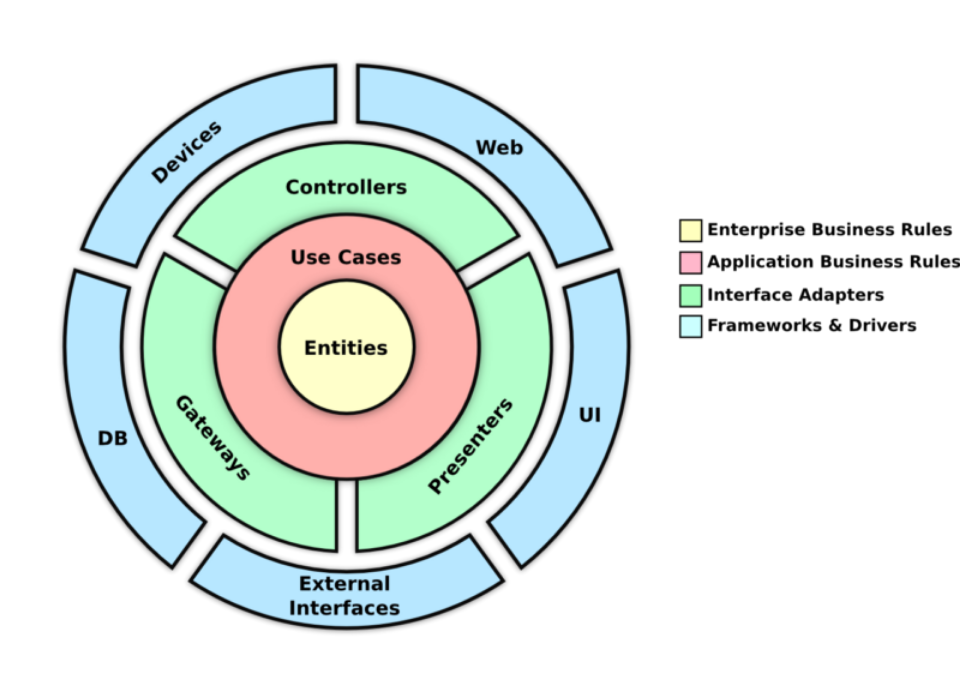
\includegraphics[width=0.6\textwidth]{c2/clean_architecture.png}
	\caption{Structură arhitecturii \textit{Clean code}}
\end{figure}

Adoptarea acestui tip de arhitectură împreună cu cea de tip \textit{monolith} include mai multe beneficii cum ar fi:

\begin{itemize}

	\item mentenanța sporită datorată faptului că modulele sau straturile principale ale aplicației și logica ce le facilitează comnunicarea eficientă sunt separate, încurajând astfel și o înțelegere mai detaliată și simplificată a întregului sistem;
	
	\item flexibilitate din punct de vedere al schimbării tehnologiilor exterioare, stratul de logică internă este independent de ceea ce se întâmplă în exteriorul său;
	
	\item testarea componentelor se poate face atât individual cât și în relație cu alte module, astfel eliminând nevoia de testare a întregii aplicații;
	
	\item stratul de logică internă este independent de baza de date folosită, asftel serverul de stocare al datelor poate fi schimbat cu ușurință.

\end{itemize} 
Modul în care arhitectura de tip \textit{Clean Code} a fost implementată în aceste proiect constă în separarea straturilor aplicației, astfel încât avem:

\begin{itemize}
	\item  \textit{Core Layer} fiind Structură principală ce conferă logica internă a aplicației. Acesta cuprinde \textit{Domain} unde sunt modelate entitățile aplicației respectiv \textit{Application} unde este definită toată logica internă a serverului,
	de la declarațiile abstracte ale interfațelor la definerea serviciilor proprii de care se vor folosi ulterior straturile externe ale arhitecturii;
	
	\item \textit{API Layer} este partea structurală care definește \textit{endpoint-urile} aplicației prin diferite \textit{controllere}, expunând astfel funcționalitățile aplicației la internet;
	
  	\item \textit{UI Layer} definește Structură de prezentare a aplicației și este formată din partea de \textit{Frontend} a platformei;
  
 	 \item \textit{Infrastructure Layer} în care găsim logica ce se ocupă de comunicarea cu serviciile externe cum ar fi baza de date, AWS sau servicii de identitate.
 	 
\end{itemize}

\subsection*{\textit{Design pattern-uri} utilizate}

\textit{Design pattern-urile}, potrivit definiției, sunt soluții generale și reutilizabile asupra problemelor comune ce pot apărea în decursul dezvoltării unei aplicații software.

Utilizarea lor conduce la o buna mentananță a codului scris, posbilitatea de a reutiliza module deja scrise, îmbunătațește comunicarea și legăturile dintre module și încurajează un stil de cod cât mai elegant și ușor de înțeles.\\
În implementarea aplicației au fost folosite \textit{desing pattern-uri} din diferite categorii astfel încât în această subsecțiune se vor discuta câteva exemple utilizate.

\subsection*{\textit{Optional pattern}}
Acesta este un model de proiectare care ajută la gestionarea valorilor care pot sau nu fi prezente, astfel având valoarea \textit{null}. \textit{Pattern-ul} se asigură că este eliminată valoarea \textit{null}, care de cele mai multe ori este o sursă comună în erori la rularea codului (\textit{runtime}).

Soluția prezentată de acest model este crearea unei clase \textit{template} care incapsulează valoarea propriu zisă a entității pe care o construim. Spre exemplu, în cazul în care vrem să creăm o nouă entitate de tipul \textit{User} dar la \textit{runtime} apare o eroare, executia programului nu se va opri, iar valoarea entității va fi incapsulată într-un tip   \textit{Result\textless User\textgreater} cu parametrul \textit{Succes} setat pe fals, indicând astfel că procesul de creare a eșuat.\\

\begin{figure}[h]
	\centering
	
	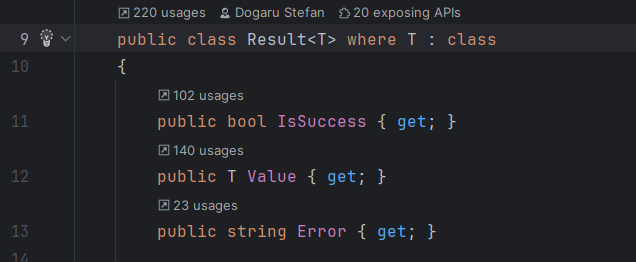
\includegraphics[width=0.8\textwidth]{c2/optional_patterns}
	\caption{Exemplu de clasă care implementează Optional Pattern}
\end{figure}

\subsection*{\textit{Mediator pattern}}
Acest \textit{design pattern} este unul de tip comportamental și se asigură că nu există dependențe haotice între entitățile/clasele din codul scris. Modelul restrictionează comunicarea directă între obiecte și le obligă să interacționeze doar prin intermediul unui \textit{mediator}.

Acest model este implementat prin utilizarea unei interfațe sau clase abstracte care știe toate referințele la componentele care vor să comunice. În acest mod, în loc să trimită solicitări directe, un obiect comunică prin intermediul mediatorului, acesta știind unde să redirecționeaze cererea primită.


\begin{figure}[h]
	\centering
	
	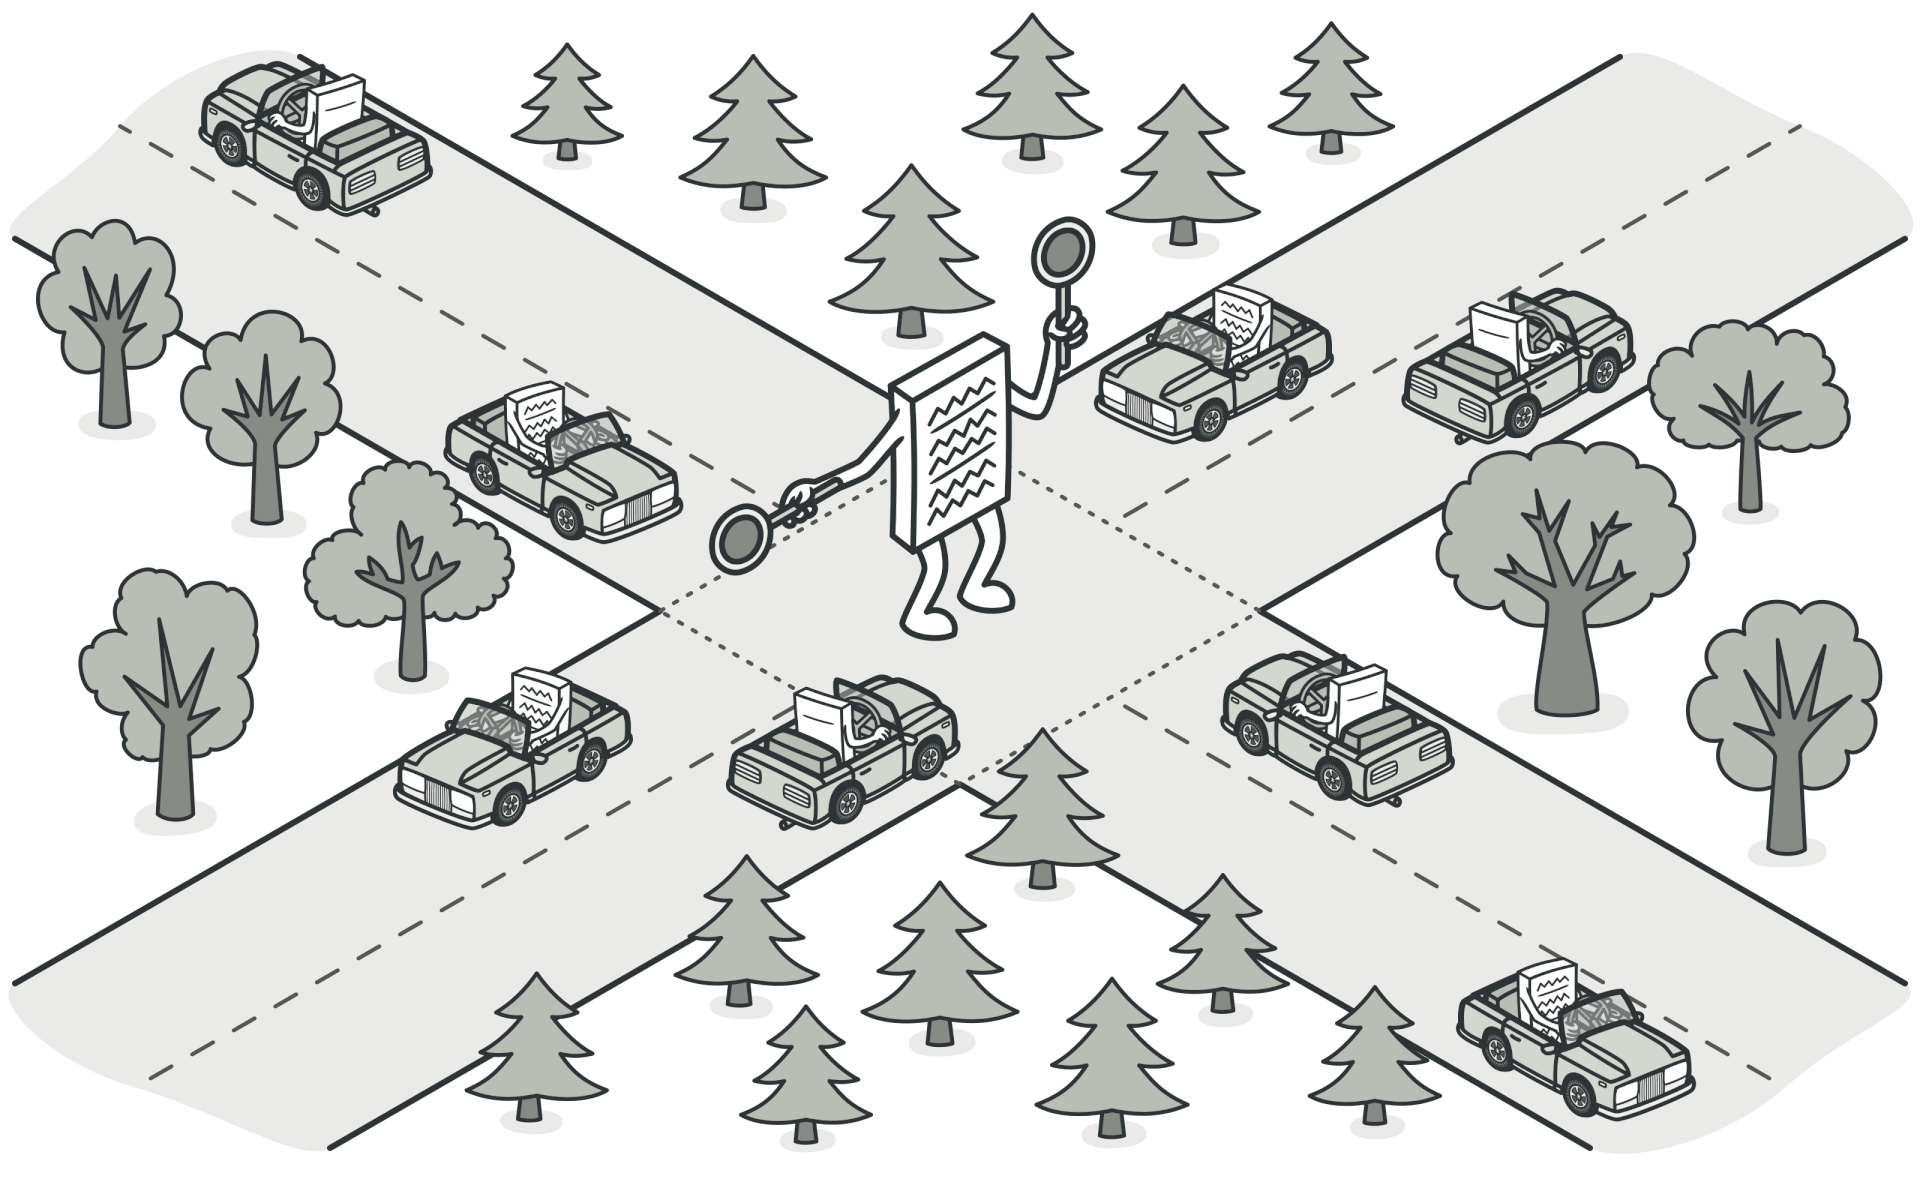
\includegraphics[width=0.6\textwidth]{c2/mediator_pattern}
	\caption{Ilustrație \textit{mediator pattern}}
\end{figure}

	\newpage
\subsection*{\textit{Command pattern}}	

Acest \textit{design pattern} este de asemenea unul de tip comportamental și se utilizează parțial de \textit{design pattern-ul Mediator}, transformând astfel o comandâ, spre exemplu o cerere de creare a unei noi entități, într-un obiect independent, acesta ulterior fiind trimis către mediator și executat în \textit{handler-ul} corespunzător acestuia, de obicei numit \textit{receiver}.

În contextul dezvoltării părții de server a aplicației AudIT, acesta este utilizat, împreună cu modelul Mediator pentru a delega orice comandă (\textit{request}) primită către obiectul care știe să o execute. În acest mod, se elimină dependențe strânse între obiecte, promovând un cod cât mai bine organizat și elegant.\\

\vspace{1cm}
\begin{figure}[h]
	\centering
	
	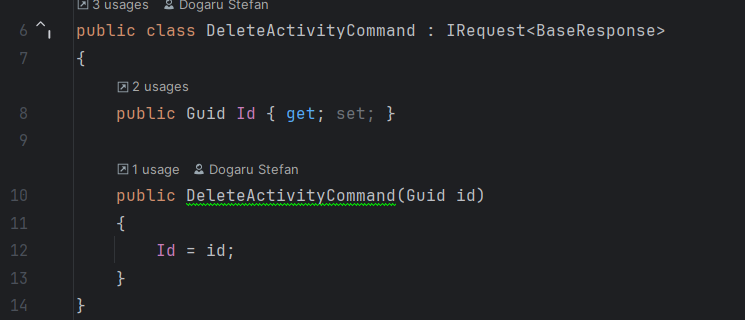
\includegraphics[width=0.7\textwidth]{c2/command_pattern1}
	\caption{Exemplu clasă de tip \textit{Command}}
\end{figure}



\vspace{1cm}
\begin{figure}[h]
	\centering
	
	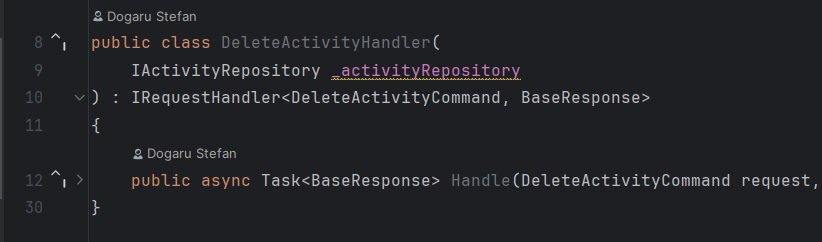
\includegraphics[width=0.7\textwidth]{c2/command_pattern2}
	\caption{Exemplu clasă de tip \textit{Handler/Receiver}}
\end{figure}


\subsection*{\textit{Repository pattern}}

Folosit în special în dezvoltarea aplicațiilor web, acest \textit{design pattern} separă logica internă a aplicației de accesul direct la date (baza de date). Acesta se utilizează de interfațe pentru a crea un strat separator între declararea abstractă a acestor constracte și implementarea concretă a funcțiilor care accesează datele la nivel de bază.

Prin acest model, comunicarea dintre module se realizează prin intermediul contractului foarte bine stabilit, astfel eliminând posibilitatea ca un modul abstract să acceseze direct un modul de acces de date.\\


\vspace{1cm}
\begin{figure}[h]
	\centering
	
	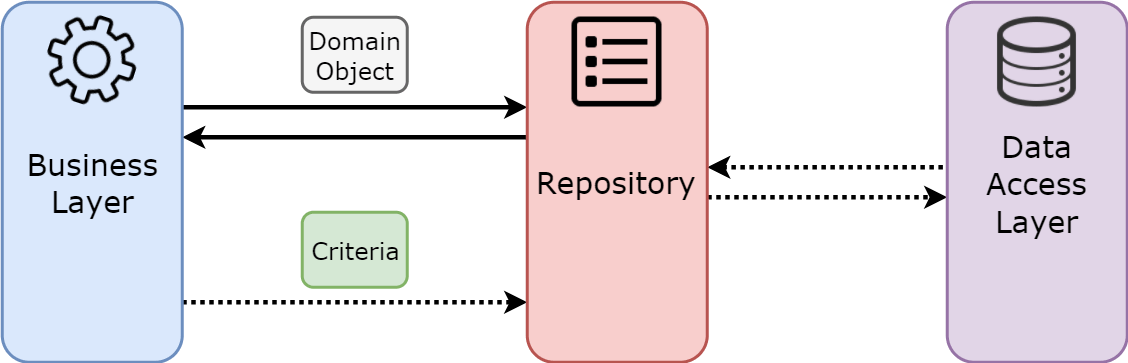
\includegraphics[width=0.8\textwidth]{c2/repository_pattern}
	\caption{Diagramă \textit{repository pattern}}
\end{figure}

\subsection*{Descriere \textit{endpoint-uri} utilizare}
\textit{Endpoint-urile} sunt componentele de bază ale comunicării aplicațiilor prin intermediul internetului și a \textit{API-urilor}. Partea de server expune informații și facilități clienților prin intermediul acestor \textit{endpoint-uri}, astfel aceștia având posiblitatea de a comunica prin intermediul acestor puncte cu aplicația și cu logica internă a acesteia.

\textit{Endpoint-urile} create de server sunt organizate conform fieăarei entități din \textit{Domeniul} aplicației , pentru o mai bună navigare și înțelgere a structurii în ansamblu, cât și având în vedere acțiunea pe care clientul dorește să o realizeze.

Principalele \textit{endpoint-uri} expuse clienților pe partea de server sunt :

\begin{itemize}
	
	\item \textit{endpoint-urile} care gestionează acțiunile utilizatorului legate de autentificare: înregistrare, autentificare, ieșire din cont, verificare email cât și actualizare a informațiilor contului de utilizator. Aceste \textit{endpoint-uri} sunt centrate în jurul entității de Utilizator;
	
	\item \textit{endpoint-urile} care se ocupă de logica gestionării entităților de tip Misiune de audit, astfel permițând crearea, listarea, ștergerea acestora cât și actualizarea informațiilor și obținerea de informații partajate cu alte entități;
	
	\item \textit{endpoint-urile} care gestionează obiectivele unei misiuni de audit;
	
	\item \textit{endpoint-urile} care tratează acțiunile unui obiectiv respectiv riscurile acestuia;
	
	\item \textit{endpoint-urile} care administrează acțiunile referitoare la entitățile de tip Recomandare;
	
	\item punct de accees asupra entităților de tip Document, existând posibilitatea de a crea, a încărca, descărca și a sterge documente salvate pe platformă;
	
	\item \textit{endpoint-urile} care gestionează acțiunile de export de date și de autocompletare a unor documente de tip șablon cu date de pe platformă;
	
	\item \textit{endpoint-urile} care permit configurarea instituțiilor și a departamentelor de pe platformă.
	
\end{itemize} 

De asemenea, \textit{server-ul} expune prin intermediul altor \textit{ endpoint-uri} funcționalități cum ar fi configurarea accesului la resurse partajate, gestionarea activităților desfășurate pe platformă cât și un sistem de notificări ce permite actualizarea informațiilor disponibile pe aplicație în timp real.


	
 

\subsection*{Tehnologii utilizate}
În dezvoltarea părții de server s-a utilizat \textit{framework-ul } ASP.NET Core împreună cu limbajul C\#.\\
Alegerea făcută se bazează pe faptul că \textit{framework-ul} este unul de tip \textit{open-source}, dezvoltat în principal de Microsoft, un actor important pe piața actuală IT,\textit{framework-ul} oferind funcționalități robuste și eficiente pentru dezvoltarea aplicațiilor web, acestea putând fi rulate pe Windows, Linux cât și MacOS.

De asemenea, C\# este un limbaj de programare multi-paradigmă \textit{high-end} matur, care oferă diverse funcționalități și solutii foarte bine puse la punct atat din punct de vedere al eficientei cât și al sustenabilitatii codului.

Mai mult de atat, integrarea celor două tehnologii cu alte servicii Microsoft este una foarte ușor de realizat, acest lucru aducănd un motiv în plus în alegerea facută, pe langă ecosistemul bogat din care acestea fac parte, oferind suport pentru o gamă largă de biblioteci și unelte deja integrate în funcționalitățile limbajului și a \textit{framework-ului}.

În plus, s-au utilizat diferite biblioteci pentru dezvoltarea anumitor servicii, cum ar fi :
\begin{itemize}
	\item  AWSSDK.Core pentru integrarea serviciilor AWS de trimitere a a unui email sau de stocare a datelor și a fișierelor în S3 Bucket;
	
	\item  MediatR care oferă funcționalitățile \textit{design pattern-ului} Mediator;
	
	\item ASP.NET Identity, serviciu pentru integrarea funcționalităților de autentificare și autorizare în aplicație, facilitănd accesul și autorizarea utilizatorilor pe platformă;
	
	
	\item AutoMapper este o bibiliotecă externă utilizată pentru a transforma diferitele tipuri de obiecte între ele, eliminănd astfel codul \textit{boilerplate} necesar pentru a copia datele de la o entitate la alta;
	
	\item OpenXML este o bibliotecă \textit{open-source} care permite manipularea fișierelor Office de tipul .XLSX sau .DOCS. Este integrată pentru a oferi utilizatorilor funcționalitatea de a putea edita sau exporta pe platformă documente oficiale tip șablon.
	
\end{itemize}
   

\section{Arhitectura interfatei grafice}
Interfața grafică dezvoltată în acest proiect este realizată în \textit{framework-ul} .NET Blazor, mai exact o aplicație de tipul \textit{WASM (Web Assembly)} care rulează în \textit{browser-ul} utilizatorului. Alegerea a fost facută întrucât acest nou model arhitectural permite rularea codului direct în \textit{browser}, nemaifiind nevoie de librării sau extensii suplimentare necesare.\\

\newpage
\subsection*{Web assembly} 
Cum se poate da seama și din numele pe care această tehnologie o poartă, este vorba despre \textit{byte-code} (cod-mașină) care este executat de o componentă separată din \textit{browser}, numită \textit{Wasm engine}.

\textit{Wasm} nu este un limbaj, ci mai degrabă produsul compilării codului scris într-un limbaj de programare în cod-masină executabil. Majoritatea limbajelor de programare moderne  suportă compilarea codului direct într-un fișier  binar de tip .wasm . După o compilare cu succes, fișierele binare .wasm sunt încărcate în \textit{browser} cu ajutorul Javascript, urmând să fie executate de către componenta menționată într-o instanță virtuală izolată și securizată.\\

\vspace{1cm}
\begin{figure}[h]
	\centering
	
	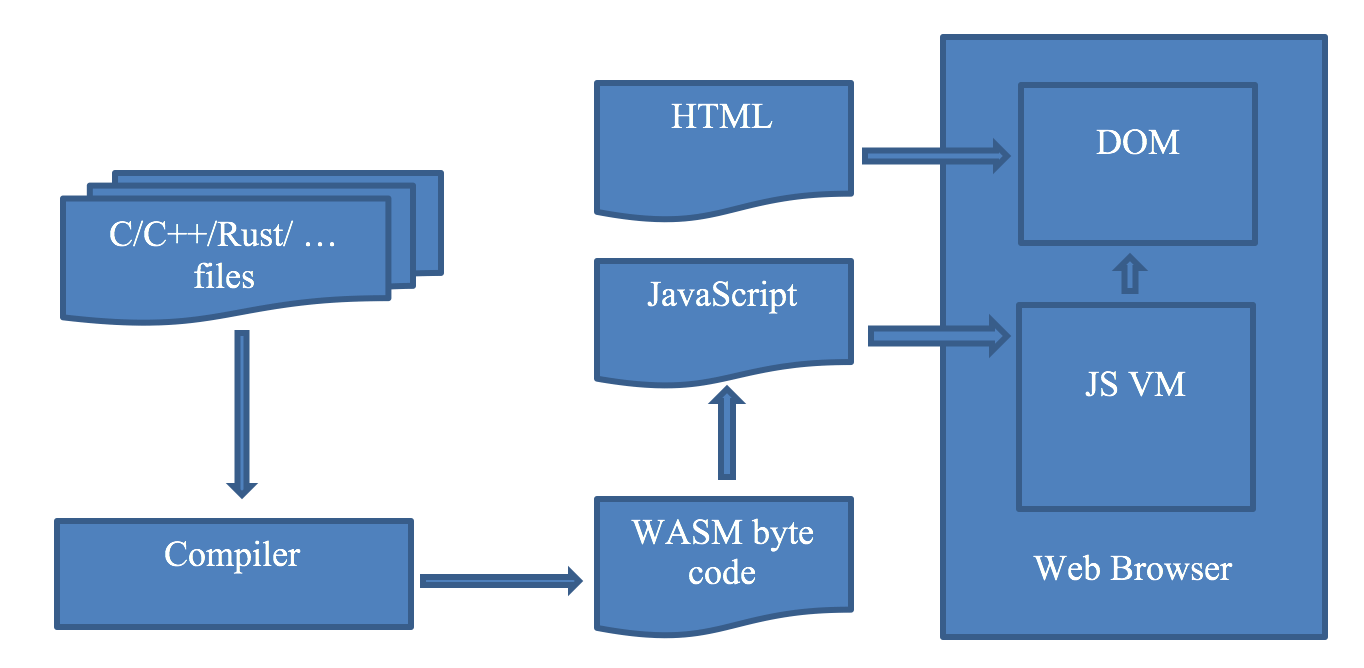
\includegraphics[width=0.7\textwidth]{c2/wasm}
	\caption{Diagrama mod functionare \textit{Web Assembly}}
\end{figure}

Un avantaj cheie al utilizarii acestei tehnologii îl constituie viteza și eficiența de care dă dovadă. Codul rulează cât se poate de aproape de limitările \textit{hardware} ale computer-ului, astfel rezultând în performanțe crescute și un nivel al utilizării memoriei mai mic.

Pe de altă parte, există și dezavantaje în utilizarea acestuia, intrucat momentan nu este implementat un sistem de \textit{garbage collector} care să elimine din memorie funcțiile și instanțele care nu mai sunt folosite în firul execuției.

\subsection*{.NET Blazor}
Pentru dezvoltarea paginilor web, s-a utilizat tehnologia .NET Blazor, un \textit{framework} relativ nou apărut, dar care promite performanțe crescute alături de un mediu de lucru bine pus la punct și eficient din punct de vedere al productivității dezvoltării interfațelor interactive și bogate.

Paginile web create în acest mod combină codul C\# cu HTML pentru a crea componente reutilizabile ce sunt  afișate și actualizate în DOM-ul virtual din \textit{browser}.\\

\vspace{1cm}
\begin{figure}[h]
	\centering
	
	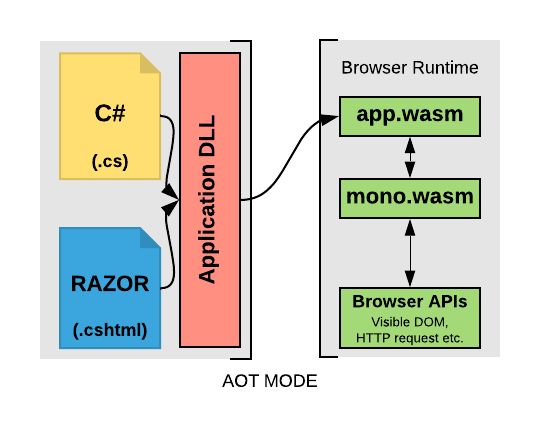
\includegraphics[width=0.7\textwidth]{c2/blazor}
	\caption{Diagrama mod functionare \textit{Blazor WebAssembly}}
\end{figure}

O funcționalitate foarte importantă pe care o oferă, este utilizarea componentelor, părți fundamentale care împreună alcătuiesc pagina web afișată utilizatorului. O componentă poate fi vazută ca o piesă esențială de puzzle care contribuie la afisarea finală a unei pagini web, piesă de puzzle care la rândul său poate fi creată din mai multe astfel de componente, și asa mai departe.

Un avantaj pe care Blazor îl oferă dezvoltatorilor este acela că elimină pe cât posibil utilizarea de funcții și \textit{script-uri }JavaScript în crearea paginilor web. Blazor se folosește de cod scris în C\# împreună cu HTML și CSS pentru a elabora pagini și componente web interactive și fluide.\\

\subsection*{Radzen Components}
De asemenea, pentru o stilizare și o reutilizare a componentelor, s-a folosit librăria Radzen Components pentru a reutiliza controale și componente cum ar fi : tabele, butoane stilizate, teme grafice de înaltă calitate, \textit{form-uri} și multe altele.

Librăria Radzen Components este una de tip \textit{open-source} și oferă suport dedicat din partea comunității active, împreună cu documentația detaliată asupra tuturor funcționalităților oferite.


\section{Stocarea datelor}

 \subsection*{Baza de date MySQL}
	MySQL este un sistem de gestionare a bazelor de date relaționale open-source și reprezintă alegerea pentru care s-a optat a fi folosită pentru stocarea datelor în proiect. Acest sistem este una dintre cele mai populare soluții când vine vorba de stocare într-un mod relațional al datelor, astfel încât acesta oferă diferite beneficii: 
	\begin{itemize}
		
		\item simplitatea când vine vorba de utilizarea acestuia, folosindu-se de un dialect comun în interogările sale, este foate ușor de utilizat;
		
		\item securitatea datelor oferită de MySQL prin integrarea unui sistem solid de privilegii și de restricționare a accesului bazat pe roluri;
		
		\item flexibilitatea și funcționalitățile pe care aceasta le oferă sporesc productivitatea dezvoltării aplicațiilor.
		
	\end{itemize} 
 
 \subsection*{Entity Framework Core}
Entity Framework Core este o tehnologie dezvoltată de Microsoft în cadrul \textit{framework-ului} .NET Core care permite dezvoltatorilor să interacționeze cu entitățile și tabelele din baza de date prin intermediul obiectelor, eliminând astfel necesitatea de a scrie interogări clasice pentru a comunica facil cu baza de date și cu obiectele sale.

Aceasta tehnologie dispune de o serie de caracteristici și funcționalități care o fac o alegere crucială în ceea ce privește comunicarea într-un mod eficient cu baza de date:
\begin{itemize}
	
	\item sistemul de \textit{migrații} similar unui \textit{version-control} al versiunii bazei de date și a relațiilor acesteia, permite dezvoltatorilor să țină evidența versiunii bazei de date, eventual existând posibilitatea în cazul unor erori să se întoarcă la ultima versiune stabilă;
	
	\item \textit{code-first} este funcționalitatea ce permite actualizarea modelului din baza de date pe baza schimbărilor din codul scris și a modificărilor din entitățile declarate în codul sursă;
	
	\item suportul pentru majoritatea bazelor de date existente în momentul de față, primind constant actualizări;
	
	\item performanța interogărilor, astfel încat sistemul este optimizat să colecteze într-un mod eficient rezultatele interogărilor.
	 
\end{itemize}

\subsection*{Structură bazei de date}

Pentru autentificarea și autorizarea activităților utilizatorilor, se utilizează biblioteca .NET Identity Core, care pune la dispoziția dezvoltatorilor o soluție deja implementată în materie de tabele și a relațiilor dintre ele, astfel încat dezvoltatorul să se ocupe doar de logica utilizării acestora.
 
\vspace{1cm}
\begin{figure}[h]
	\centering
	
	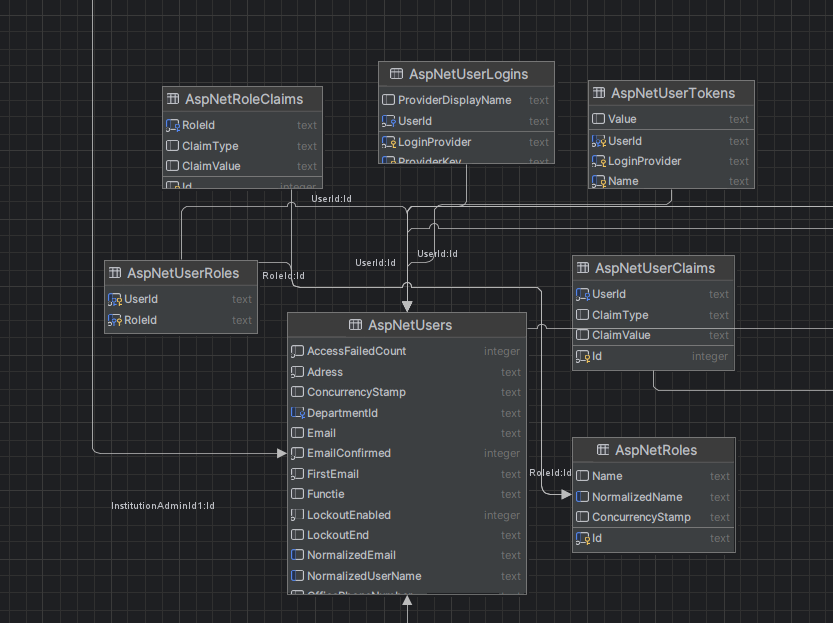
\includegraphics[width=1\textwidth]{c2/db1}
	\caption{Structură tabele autentificare și autorizare}
\end{figure}

Pentru organizarea și dezvoltarea funcționalităților în ceea ce priviște misiunile de audit, sunt o serie de tabele care gestionează misiunile de audit, obiectivele acesteia, recomandările aduse cât și documentele asociate cu respectiva misiune de audit.

\vspace{1cm}
\begin{figure}[h]
	\centering
	
	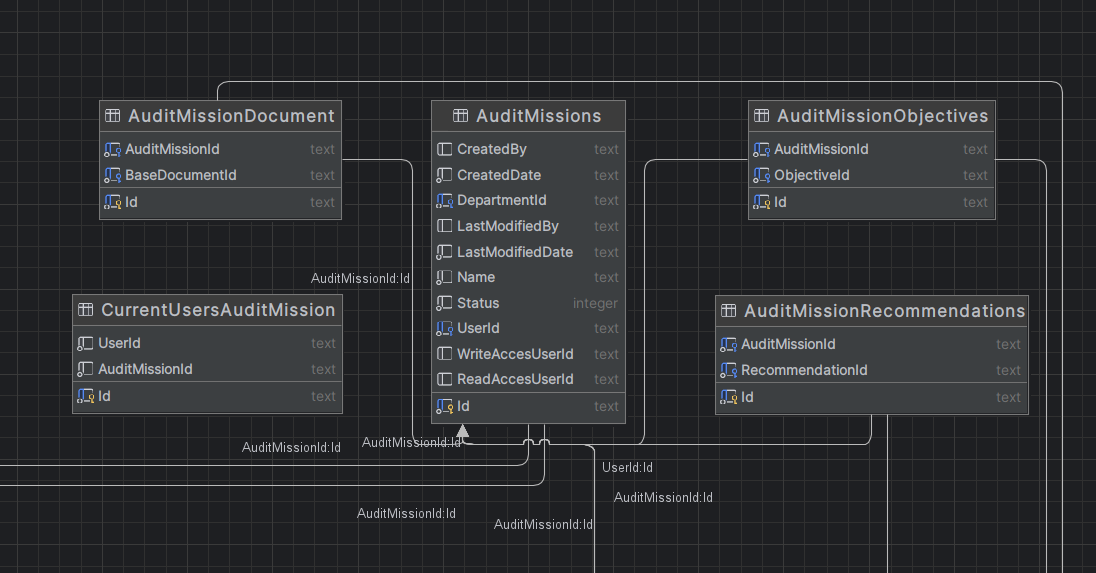
\includegraphics[width=1\textwidth]{c2/db2}
	\caption{Structură tabele gestiune misiuni de audit}
\end{figure}

\newpage
Pentru gestionarea instituțiilor și a departamentelor acestora, cât și a documentelor de baza ce aparțin acestora se folosec urmatoarele tabele și relațiile dintre ele.
\vspace{1cm}
\begin{figure}[h]
	\centering
	
	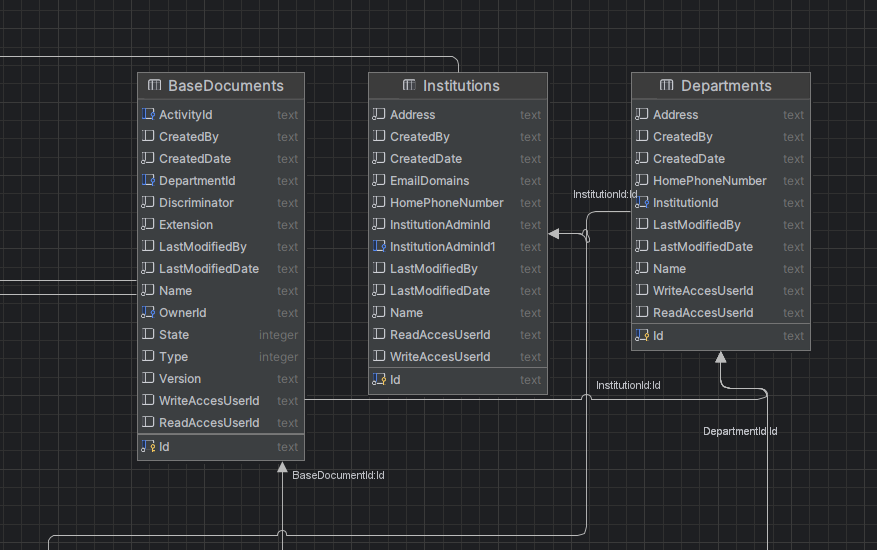
\includegraphics[width=1\textwidth]{c2/db3}
	\caption{Structura tabelelor de gestiune a institutiilor și a departamentelor}
\end{figure}

În cele din urmă, pentru oferirea funcționalităților principale, cum ar fi gestionarea obiectivelor, a acțiunilor acestora precum și a riscurilor și recomandărilor se utilizează următoarele tabele și relații pe care acestea le prezintă.

\vspace{1cm}
\begin{figure}[h]
	\centering
	
	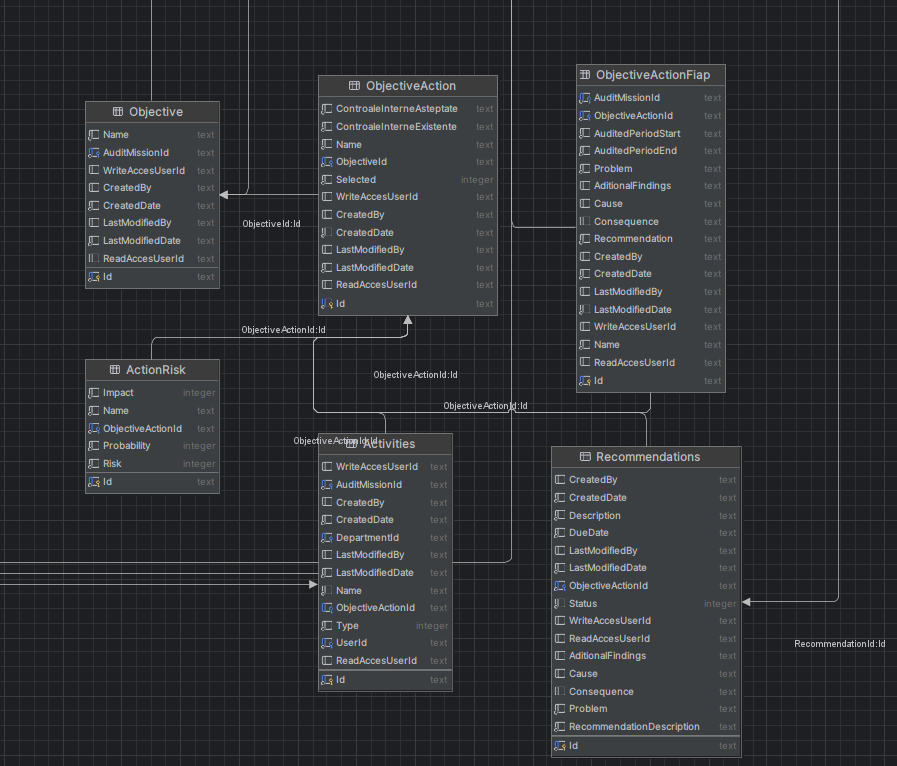
\includegraphics[width=1\textwidth]{c2/db4}
	\caption{Structura tabelelor funcționalități principale}
\end{figure}

\section{Aspecte de securitate}

Simpla dezvoltare a unei aplicații web ce oferă utilizatorului numeroase funcționalități nu este suficientă dacă această aplicație nu dispune de un set de reguli și aspecte ce  fac experiența utilizatorilor pe platformă una cât mai sigură, în care le este asigurată integritatea, confidențialitatea cât și disponibilitatea datelor și actiunilor acestora.

În dezvoltarea platformei AudIT s-a încercat utilizarea a cât mai multor standarde în ceea ce priveste securitatea acțiunilor pe care un potențial utilizator poate să le facă în aplicație, precum și a datelor și informațiilor cu care acesta lucrează.

\subsection*{Autentificarea actiunilor}

Atat pe partea de server cât și în cea de client, sunt implementate funcționalități ce previn utilizarea \textit{endpoint-urilor} și accesarea paginilor web când un utilizator nu este autentificat pe aplicație. Mai mult de atat, accesul la anumite funcționalități este restricționat doar unor categorii de utilizatori, cu un rol specific, astfel un utilizator cu rolul de reprezentant al unei instituții nu va putea accesa paginile specifice creării și actualizării unei misiuni de audit, întrucat rolul pe care acesta îl detine nu are nivel de permisiune necesar pentru această acțiune.

Modalitatea prin care este verificată este prin atribuirea unui \textit{token} de tip JWT (\textit{JSON web token}) fiecărui utilizator în momentul în care acesta se autentifică pe platformă, ulterior la fiecare acțiune (\textit{request}) facută de acesta, fiind trimis și acest \textit{token}.\\



\textbf{Stocarea} acestui \textit{token} de acces se face într-o manieră securizată în \textit{browser-ul} clientului sub forma unui \textit{cookie http-only}, care previne citirea acestuia de orice \textit{script} sau librărie externă din \textit{browser}, fiind utilizat doar în componența unui \textit{request} prin HTTP, astfel protejând aplicația și utilizatorii săi împotriva atacurilor de tip XSS(\textit{cross-site-scripting}).

\vspace{1cm}
\begin{figure}[h]
	\centering
	
	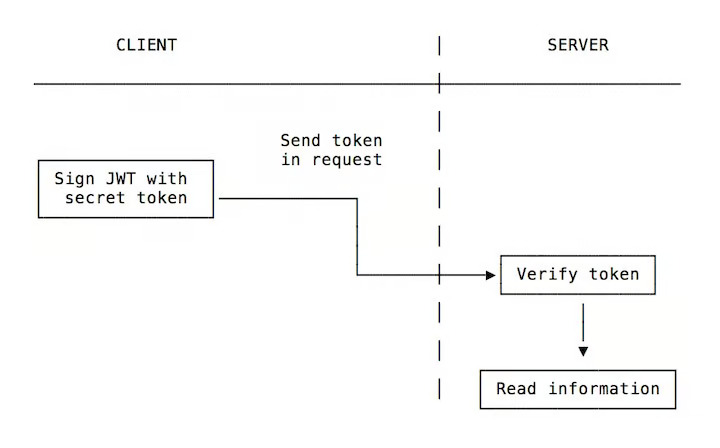
\includegraphics[width=0.7\textwidth]{c2/jwt.jpg}
	\caption{Diagramă mod functionare \textit{Web Assembly}}
\end{figure}

Pentru verificarea rolurilor și \textit{claim-urilor} pe care un utilizator le deține, este creat un \textit{endpoint} special, securizat astfel încat să poată fi accesat doar dacă în componența \textit{request-ului} este prezent acel \textit{cookie}, care oferă informatii despre rolurile și \textit{claim-urile} specifice utilizatorului care a făcut cererea. Pe baza acestora, i se permite sau i se interzice accesul la anumite pagini și acțiuni pe care acesta le dorește a face.


\subsection*{Utilizarea HTTPS}

Utilizarea HTTPS atât în partea de server, cât și în cea de client impune mai multe aspecte benefice în ceea ce priveste securitatea platformei:

\begin{itemize}
	
	\item confidențialitatea datelor, https criptează informația transmisă între server și client, astfel se asigură de faptul că șansele de interceptare și citire a  comunicației sunt aproape de zero;
	
	\item integritatea datelor este asigurată tot prin mecanismul de criptare a acestora, astfel asigurându-se de faptul că acestea ajung la destinație neschimbate;
	
	\item autententificarea, https folosindu-se de certificate digitiale (SSL și TLS) pentru a verifica identitatea serverelor, reducănd riscul unor atacuri malițioase; 
	
\end{itemize}


\subsection*{Restricționarea înregistrării pe platformă}

O altă modalitate prin care se menține un nivel ridicat de securitate pe platformă o definește restricționarea utilizatorilor de a se înregistra pe platformă.

La pasul de creare a unui cont nou, utilizatorilor le este  impusă folosirea unei adrese de email care conține domeniul unei instituții înregistrate și configurate pe platformă. Dupa crearea cu succes a unui cont nou, acesta nu are nici o permisiune, contul fiind nevoit a fi verificat de către o persoană cu drepturi elevate (administratorul instituției).

Verificarea se face pe baza unui email primit de acesta în care se cere validarea identității noului cont creat, astfel minimizând riscul creării a unor conturi false respectiv a unor false identități.

\newpage
